\documentclass[10pt]{slnotes}
\newcommand\sltilde{\char`~}
\begin{document}
\chapter{CS2106: Basic ideas}
The first computers did not have OSes. Rudimentary OSes like batch OSes that executed programs one at a time developed in the 1960s. Time-sharing OSes came in the 1970s.

OSes abstract away hardware, manage resources, control program execution and provide security and protection.

\sldef{Monolithic kernels} are kernels where the entire kernel runs in kernel mode. This design is well understood and tends to have better performance, but components tend to be more coupled and usually have complicated internal structures. Most Unices are largely monolithic.

\sldef{Microkernels} are kernels where the kernel is very small and handles only basic services like IPC, interrupt handling, and memory and task management. Higher level services run in user space, built on top of the basic facilities. This usually leads to a more robust kernel with better isolation, but performance tends to be lower.

\sldef{Layered systems} are generalisations of monolithic kernels that could be seen as a cross between microkernels and monolithic kernels: most services still run in kernel mode, but they are divided into layers, with the lowest being the hardware abstraction layer, and higher layers making use of lower layers. NT is generally seen as a layered system.

The \sldef{client-server model} is a variation of a microkernel. Servers are built on top of the microkernel and client processes request services from servers. Client and server processes can be on separate machines.

\sldef{Virtualisation} is used to run multiple OSes on the same hardware, or to debug an OS. Using a \sldef{hypervisor}, underlying hardware is virtualised. A \sldef{type 1} \sltilde{} is one that runs directly on hardware; a \sldef{type 2} \sltilde{} runs on a host OS.

\chapter{Processes}
A \sldef{process}/task/job is an abstraction to represent a program in execution.

Each \sltilde{} is represented in the system process table by a \sldef{process control block} which contains the register state (PC, SP, FP, GPRs, etc.), memory region information, PID, process state, etc.

CS2106 models processes as having 5 states: new, ready, running, blocked, and terminated.

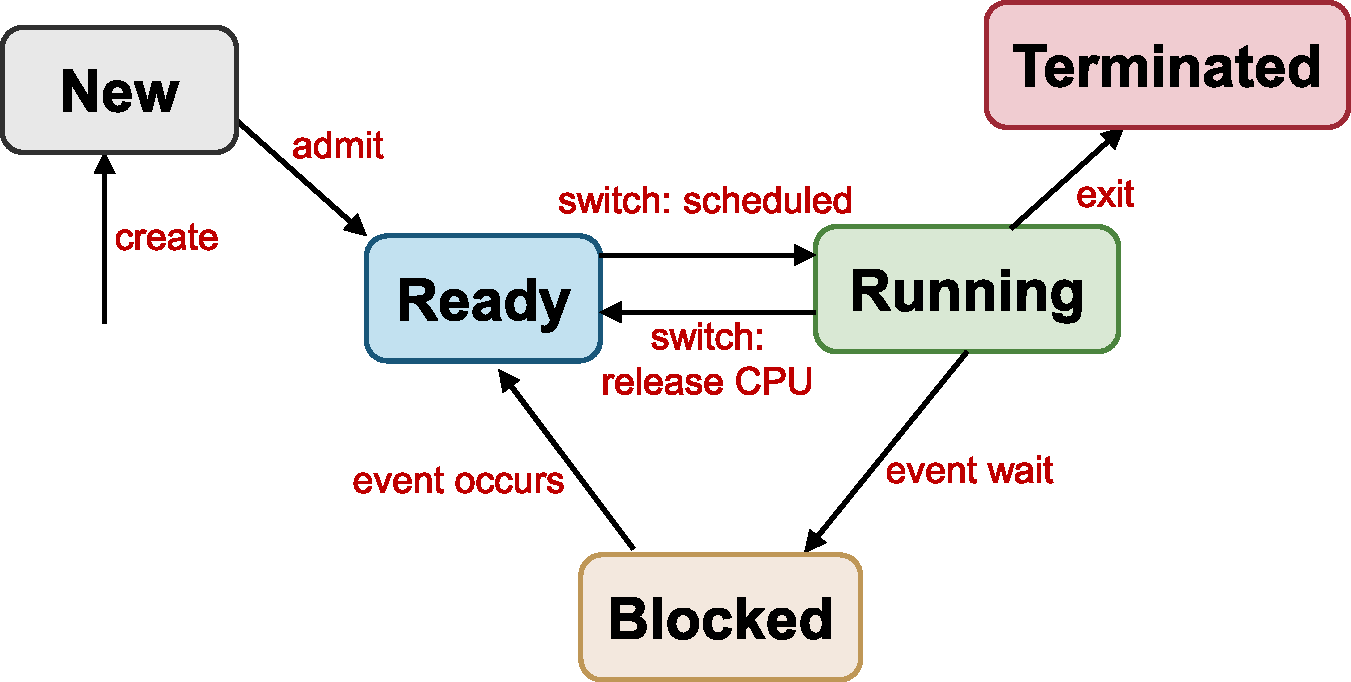
\includegraphics[width=\columnwidth]{pstates.pdf}

A \sldef{system call} is a request by a program for the system to do something. A change from user to kernel mode needs to happen. The general mechanism is \begin{slinenum}
\item program calls library
\item library performs syscall convention e.g. syscall no. in register, then execute special instruction
\item syscall entry dispatches to correct handler
\item syscall is executed
\item returns to user mode
\item library returns
\end{slinenum}.

An \sldef{exception} is a synchronous event caused by program execution e.g. arithmetic errors or segmentation faults; an exception handler (in the kernel) is executed. An \sldef{interrupt} is an external event e.g. timers or mouse/keyboard events; they are asynchronous and occur independently of program execution; program execution is suspended and an interrupt handler is executed.

Each task has a \sldef{stack} that keeps track of e.g. return address, function arguments, local variables, saved registers (register spilling when GPRs are exhausted).

A \sldef{calling convention} determines what the caller and callee does to set up the stack frame, how to pass arguments, what registers are saved by who, etc.

\section{Unix process abstraction}
\texttt{int fork()} creates a child process by duplicating the current process. Linux has \texttt{clone()} that allows more fine-grained control.

The \texttt{exec} family replaces the currently running program with a new one.

\texttt{void \_exit(int status)} ends the current process with the given status.

\texttt{pid\_t wait(int *wstatus)} waits for a child process to terminate; \texttt{pid\_t waitpid(pid\_t pid, int *wstatus, int options)} waits for (possibly) a specific child process; \texttt{waitid} waits for any child to change status.

When a process exits, it becomes a zombie process until its parent \texttt{wait()}s on it. If a process exits before child processes exit, the children will be inherited by \texttt{init}.

Linux process states: ready, running, stopped, suspended/sleeping, zombie.
\end{document}
